\documentclass[tikz, border=3.14mm]{standalone}
\usepackage{pgfplots}
\pgfplotsset{compat=1.18}
\usepgfplotslibrary{groupplots}

\begin{document}
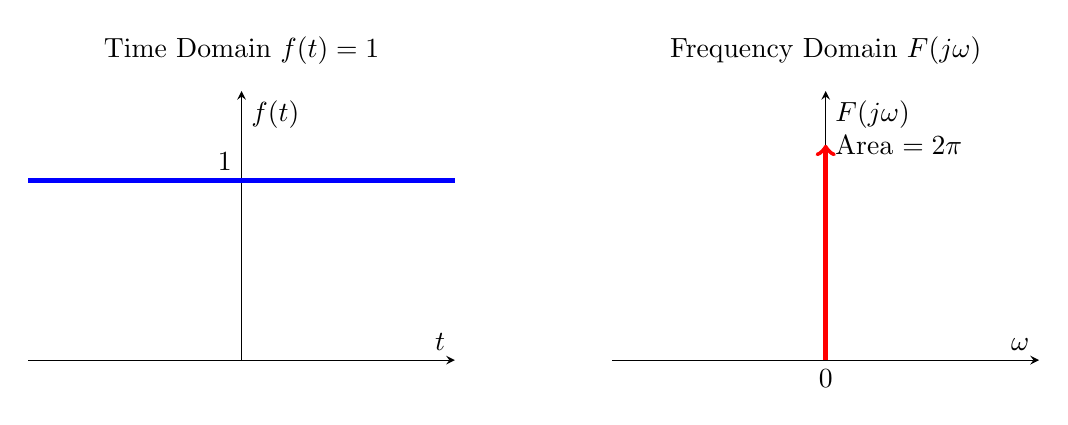
\begin{tikzpicture}
    \begin{groupplot}[
        group style={group size=2 by 1, horizontal sep=2cm},
        axis lines = middle,
        width = 7cm, height = 5cm,
        ymin = 0, ytick = \empty,
        xtick = \empty,
        grid=none
    ]
        % Time Domain
        \nextgroupplot[
            title = {Time Domain $f(t) = 1$},
            xlabel = {$t$},
            ylabel = {$f(t)$},
            xmin = -5, xmax = 5,
            ymax = 1.5,
            samples = 2
        ]
        \addplot[ultra thick, blue, domain=-5:5] {1};
        \node[anchor=south east] at (axis cs:0, 1) {$1$};

        % Frequency Domain
        \nextgroupplot[
            title = {Frequency Domain $F(j\omega)$},
            xlabel = {$\omega$},
            ylabel = {$F(j\omega)$},
            xmin = -2, xmax = 2,
            ymax = 1.5,
            xtick = \empty,
            clip = false
        ]
        \draw[->, ultra thick, red] (axis cs:0,0) -- (axis cs:0,1.2);
        \node[anchor=north] at (axis cs:0, 0) {$0$};
        \node[anchor=west] at (axis cs:0, 1.2) {Area $= 2\pi$};

    \end{groupplot}
\end{tikzpicture}
\end{document}
